\documentclass[letterpaper,9pt,twocolumn,twoside,]{pinp}

%% Some pieces required from the pandoc template
\providecommand{\tightlist}{%
  \setlength{\itemsep}{0pt}\setlength{\parskip}{0pt}}

% Use the lineno option to display guide line numbers if required.
% Note that the use of elements such as single-column equations
% may affect the guide line number alignment.

\usepackage[T1]{fontenc}
\usepackage[utf8]{inputenc}

% pinp change: the geometry package layout settings need to be set here, not in pinp.cls
\geometry{layoutsize={0.95588\paperwidth,0.98864\paperheight},%
  layouthoffset=0.02206\paperwidth, layoutvoffset=0.00568\paperheight}

\definecolor{pinpblue}{HTML}{185FAF}  % imagecolorpicker on blue for new R logo
\definecolor{pnasbluetext}{RGB}{101,0,0} %



\title{A Template for Two or One-Column Vignettes}

\author[a]{First Author}
\author[a,b]{Second Author}

  \affil[a]{Institute of Smoke and Magic, University of Sometown,
Sometown, XY, 12345}
  \affil[b]{Department of Neat Tricks, Whereever State University,
Someplace, MC, 67890}

\setcounter{secnumdepth}{0}

% Please give the surname of the lead author for the running footer
\leadauthor{Author and Author}

% Keywords are not mandatory, but authors are strongly encouraged to provide them. If provided, please include two to five keywords, separated by the pipe symbol, e.g:
 \keywords{  one |  two |  optional |  keywords |  here  }  

\begin{abstract}
Your abstract will be typeset here, and used by default a visually
distinctive font. An abstract should explain to the general reader the
major contributions of the article.
\end{abstract}

\dates{This version was compiled on \today} 


% initially we use doi so keep for backwards compatibility
% new name is doi_footer
\doifooter{\url{https://cran.r-project.org/package=YourPackage}}

\pinpfootercontents{YourPackage Vignette}

\begin{document}

% Optional adjustment to line up main text (after abstract) of first page with line numbers, when using both lineno and twocolumn options.
% You should only change this length when you've finalised the article contents.
\verticaladjustment{-2pt}

\maketitle
\thispagestyle{firststyle}
\ifthenelse{\boolean{shortarticle}}{\ifthenelse{\boolean{singlecolumn}}{\abscontentformatted}{\abscontent}}{}

% If your first paragraph (i.e. with the \dropcap) contains a list environment (quote, quotation, theorem, definition, enumerate, itemize...), the line after the list may have some extra indentation. If this is the case, add \parshape=0 to the end of the list environment.

\acknow{This template package builds upon, and extends, the work of the
excellent \href{https://cran.r-project.org/package=rticles}{rticles}
package, and both packages rely on the
\href{http://www.pnas.org/site/authors/latex.xhtml}{PNAS LaTeX} macros.
Both these sources are gratefully acknowledged as this work would not
have been possible without them. Our extensions are under the same
respective licensing term
(\href{https://www.gnu.org/licenses/gpl-3.0.en.html}{GPL-3} and
\href{https://www.latex-project.org/lppl/}{LPPL (\textgreater= 1.3)}).}

\hypertarget{introduction}{%
\section{1. Introduction}\label{introduction}}

We propose a deep-learning approach for cell classification in image
data to overcome the limitations of traditional manual cell analysis
methods for cell types. Cell analysis is crucial in various scientific
domains such as biology, medicine, and drug discovery. However, manual
methods are labour-intensive, time-consuming, and require more
comprehensive feature representation and generalizability.

Our approach holds significance for pharmaceutical companies engaged in
drug discovery and cell behaviour analysis. It aims to improve
efficiency, productivity and provide reliable cell classification
results. Consequently, this approach can lower costs and increase
profits while improving human health.

Deep learning models offer distinct advantages beyond classical machine
learning, including automated feature learning, improved generalisation
capabilities, and streamlined analysis. These models eliminate the need
for manual feature engineering by automatically learning relevant
features from raw data. This allows for more comprehensive and
expressive representations, enhancing the overall effectiveness of cell
classification.

Our study aims to address two key research questions. Firstly, we seek
to enhance the interpretability of deep learning models for cell
classification, enabling researchers to understand the underlying
patterns and features the models use. This understanding is essential
for gaining insights into the decision-making process and establishing
trust in the predictions made by the models. Secondly, we investigate
the impact of variations in training data on the performance of
different neural architectures. By systematically manipulating the
training data and evaluating model performance, we can gain valuable
insights into the robustness and adaptability of deep learning models
for cell classification tasks.

\begin{figure*}
  \begin{center}
    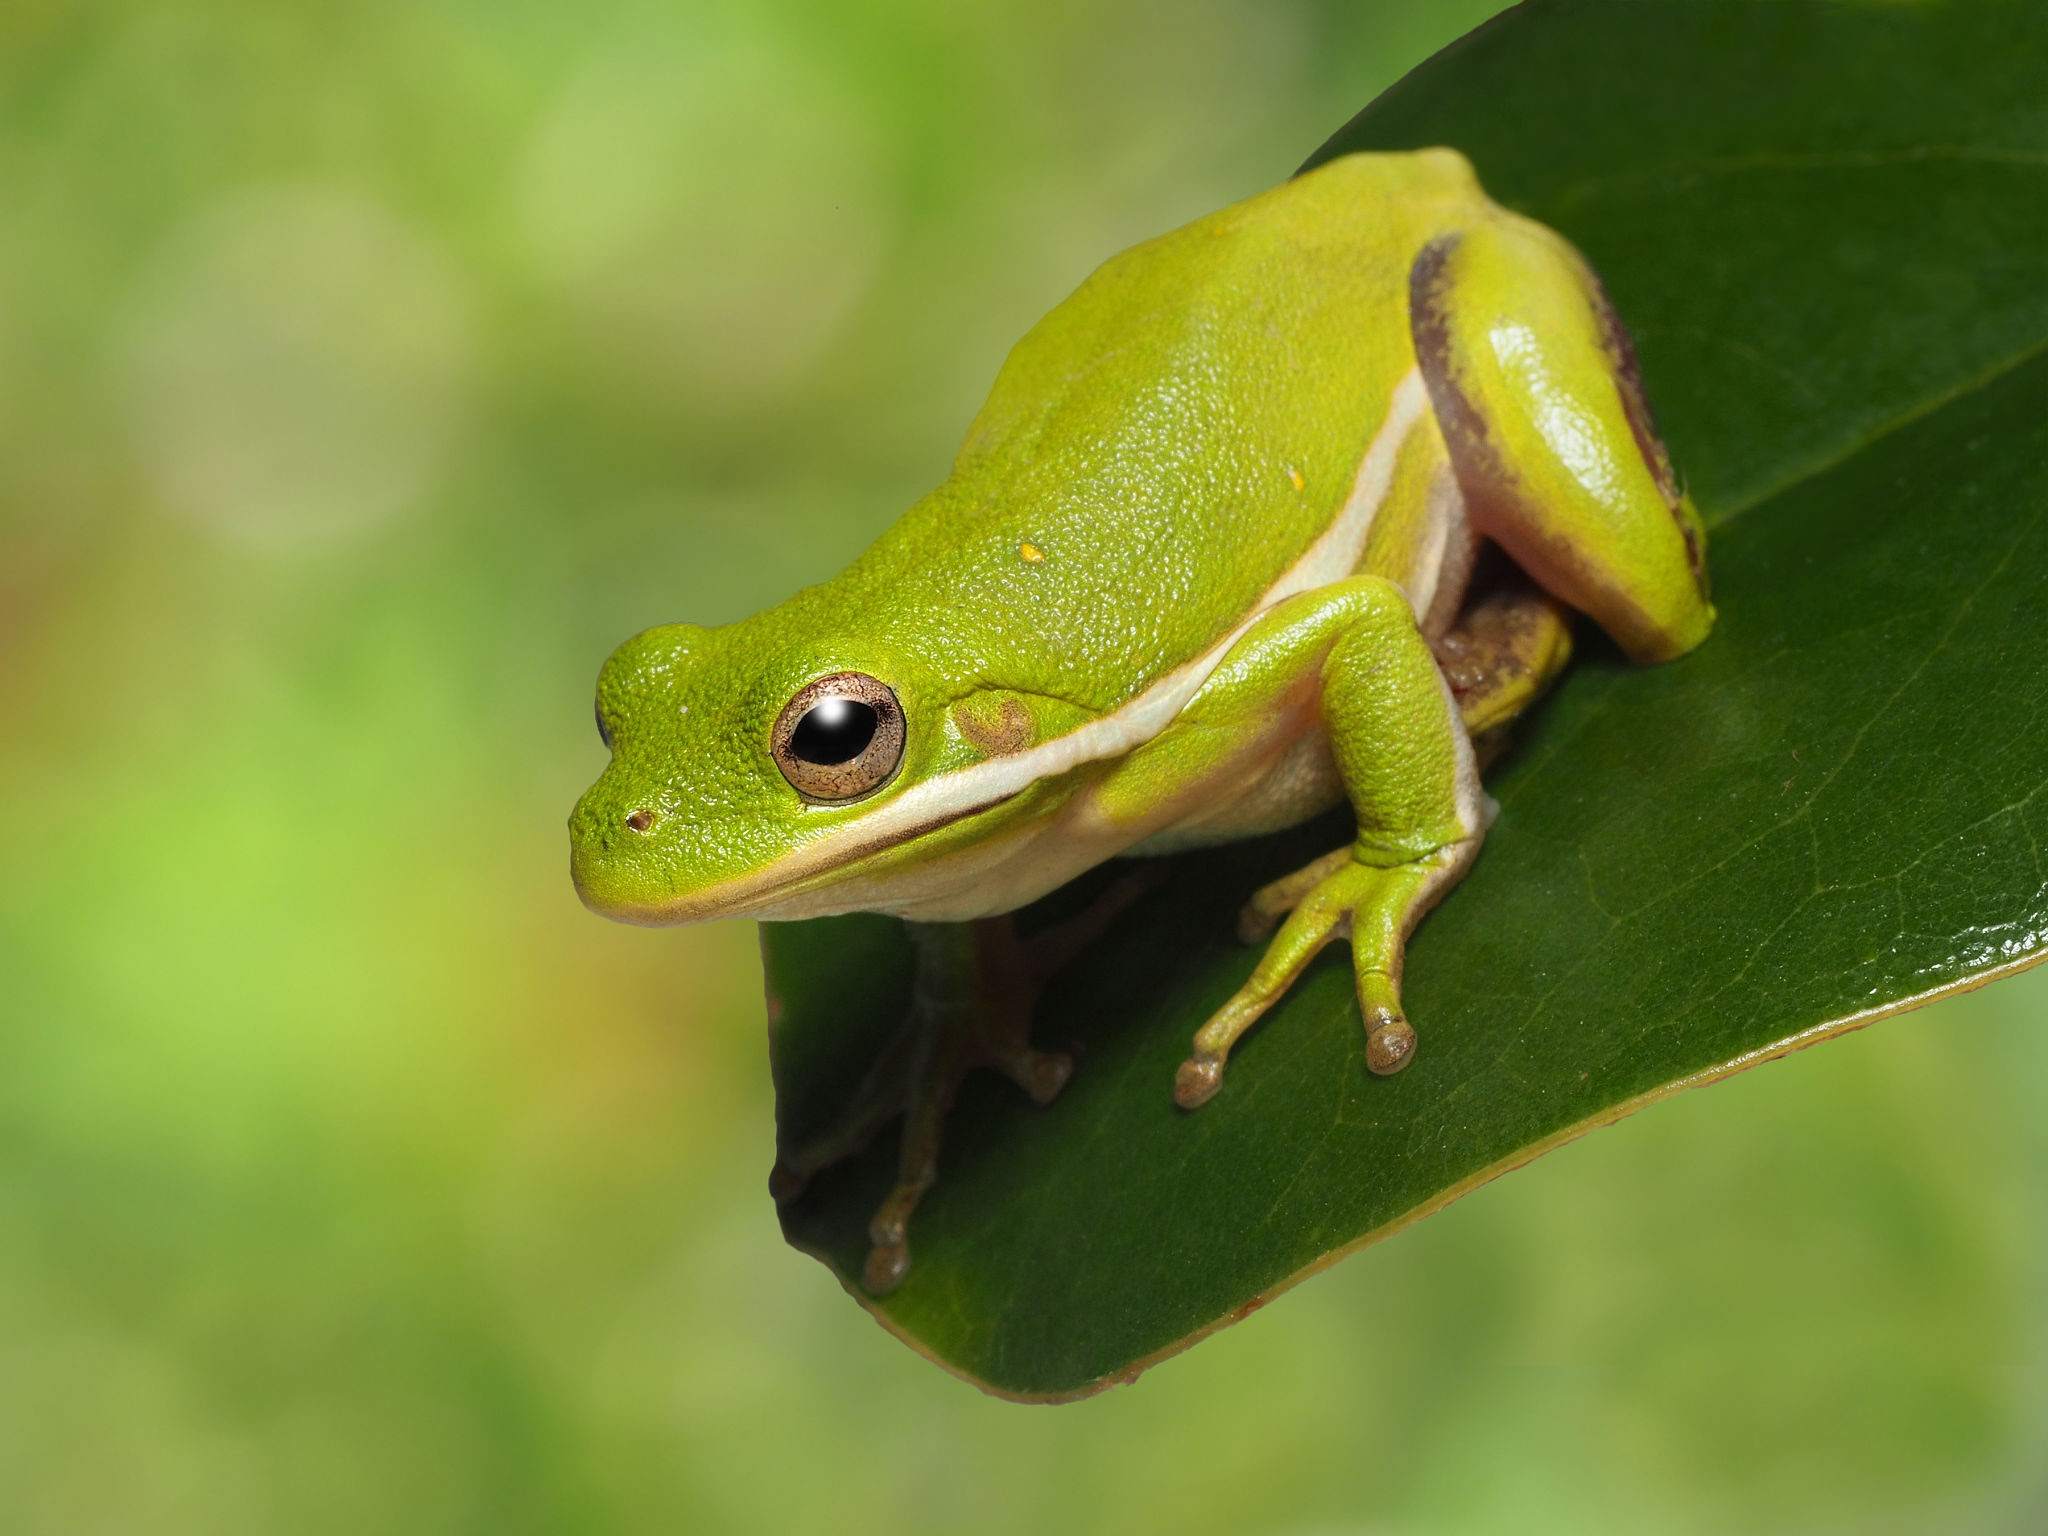
\includegraphics[width=0.66\textwidth, height=3.5in]{images/frog.png} 
  \end{center}
  \caption{Project Schematic Overview - Four key phase of project ///// I couldn't find the full resolution image for the diagram so here's a frog}\label{fig:Figure_1}
\end{figure*}

\hypertarget{methodology}{%
\section{2. Methodology}\label{methodology}}

\hypertarget{methodology-overview}{%
\subsection{2.1 Methodology overview}\label{methodology-overview}}

Figure \ref{fig:Figure_1} illustrates the research process, including
data collection, initial data analysis, data cleaning and preprocessing,
model design, training and optimisation, as well as evaluation.

\hypertarget{data-collection}{%
\subsection{2.2 Data collection}\label{data-collection}}

We obtained the data for our study from 10X Genomics (2023), consisting
of microscopy images of the mouse brain coronal section in the Tagged
Image File Format (TIFF or TIF). The gene expression levels of each cell
were categorised into 28 distinct clusters, identified by cluster IDs
ranging from 1 to 28. Hence, we obtained a CSV file with columns for
cell IDs and corresponding clusters.

We first establish a structured folder hierarchy to store the images,
with each cluster assigned a dedicated folder for its corresponding
images. This approach ensures efficient management and retrieval of the
processed data.

To extract the necessary data, we utilised information on cell
boundaries available in the dataset. Unlike our previous laboratory
work, where we only used a random sample of 1000 images, we revisited
the original dataset and extracted over 36,000 images, encompassing all
cells available. We decide to fully harness the dataset's potential and
maximise its utilisation for our analysis. We named each cell image
extracted in the ``Cell\_\{X\}'' format, where X represents the cell id,
and saved it as a PNG file in the folder of its corresponding clusters.

\newpage

\begin{figure*}
  \begin{center}
    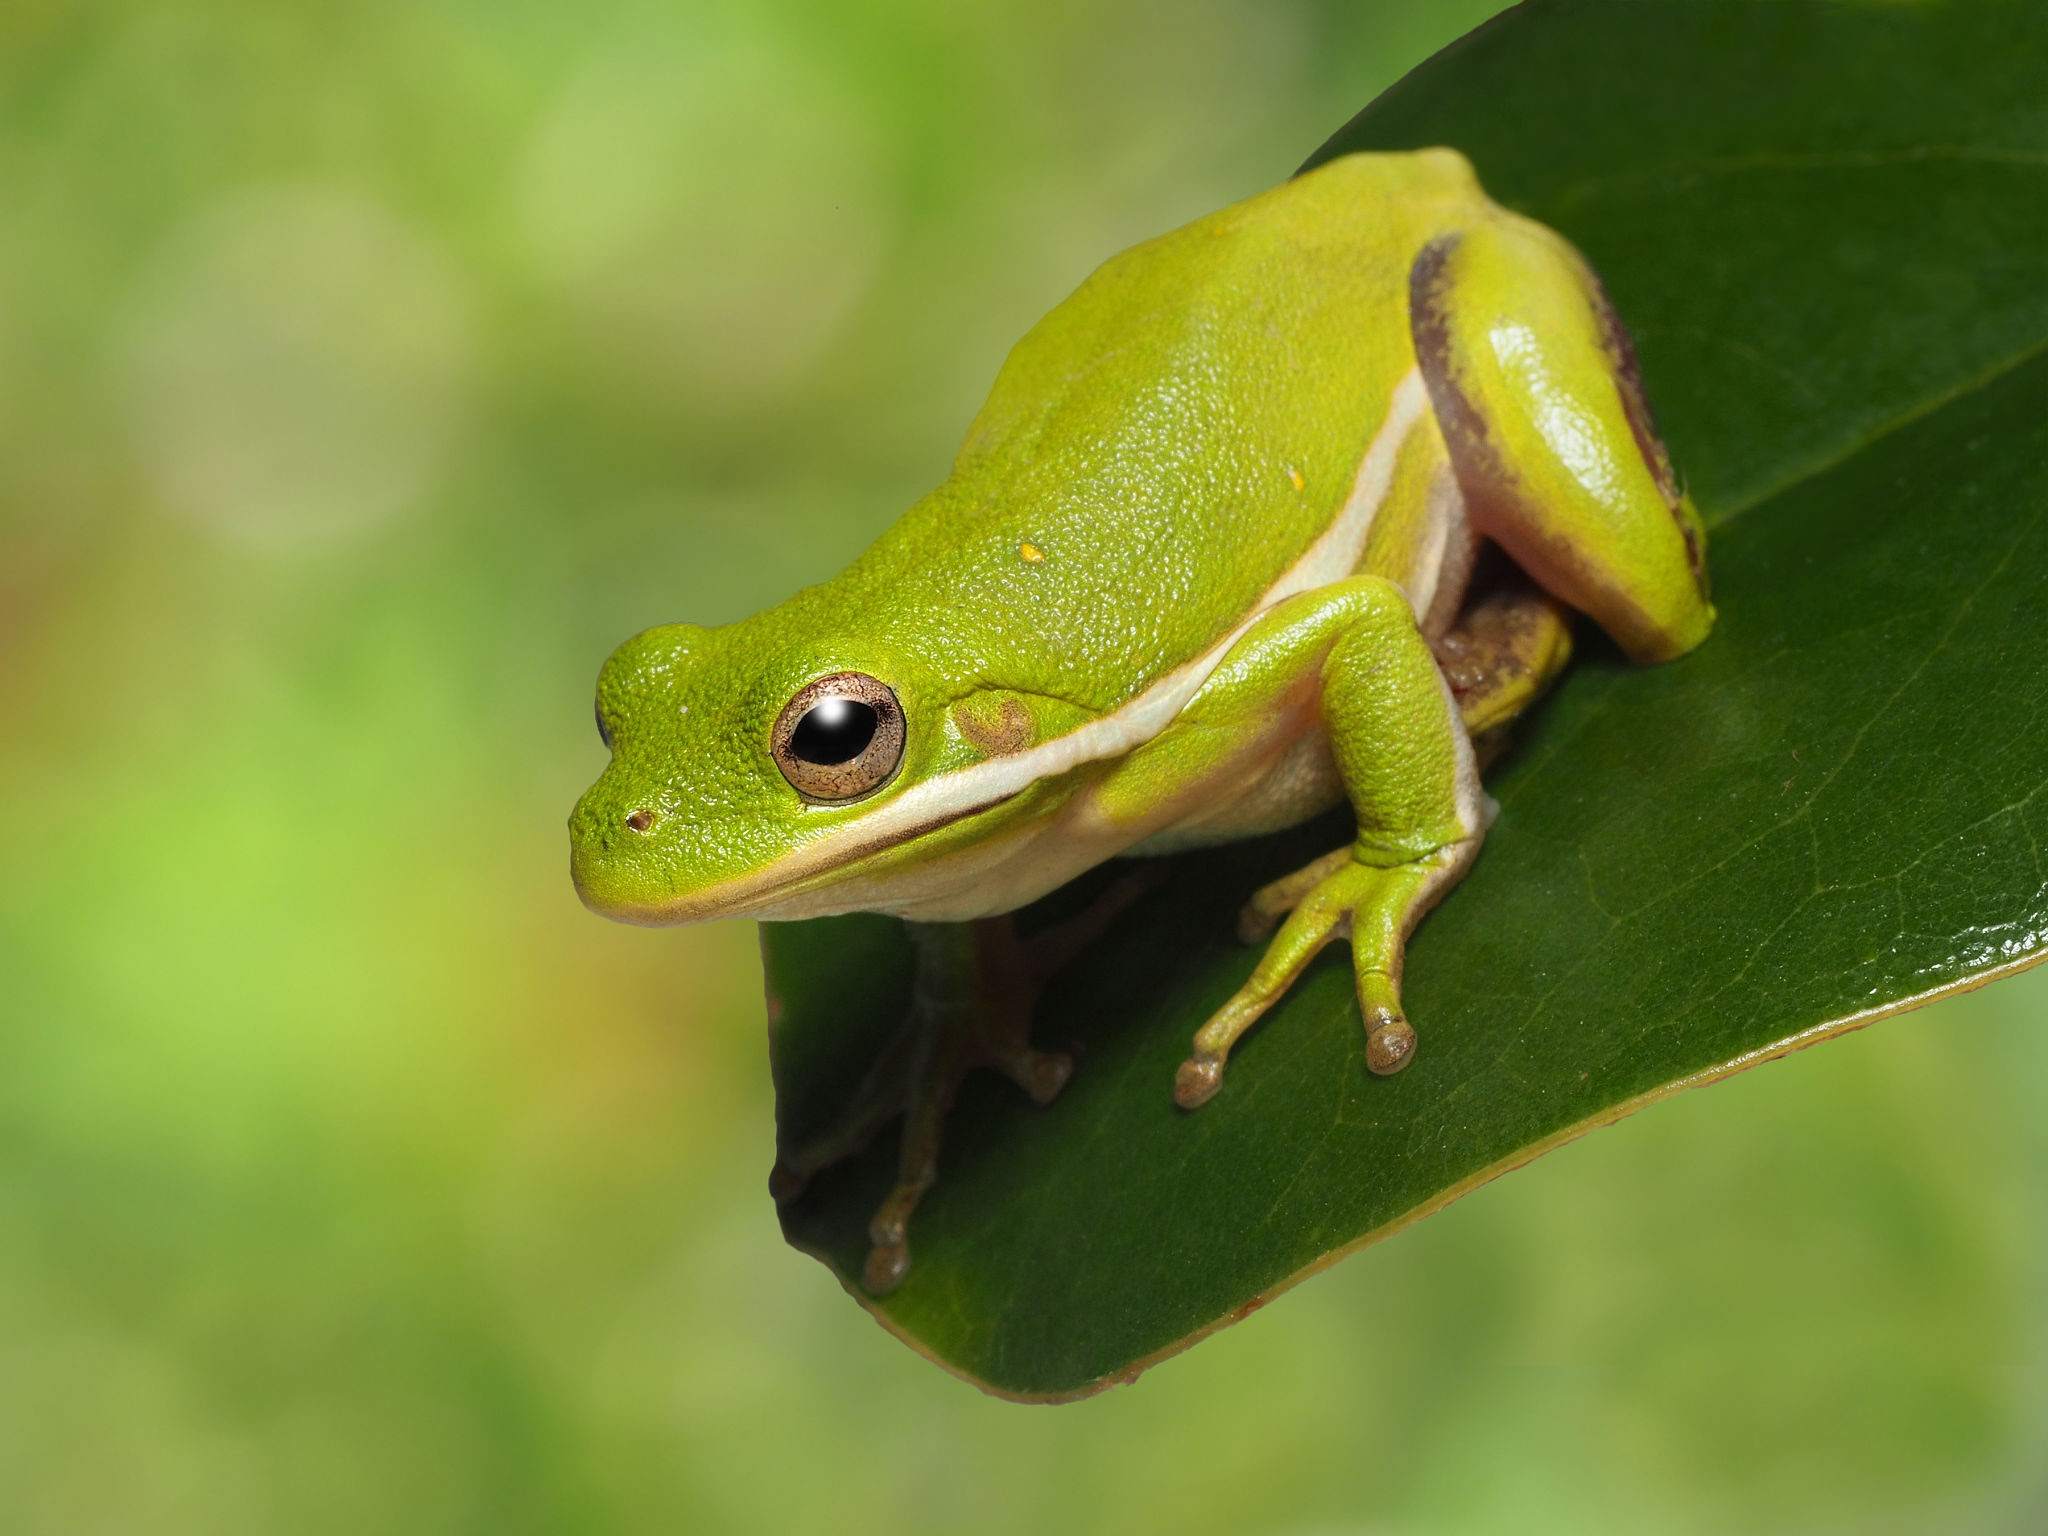
\includegraphics[width=0.4\textwidth, height=2in]{images/frog.png} 
  \end{center}
  \caption{Number of images per cluster //// This should be number of images per cluster Can't find the imageeeee, here's a frog}\label{fig:image_per_cluster}
  
  \begin{center}
    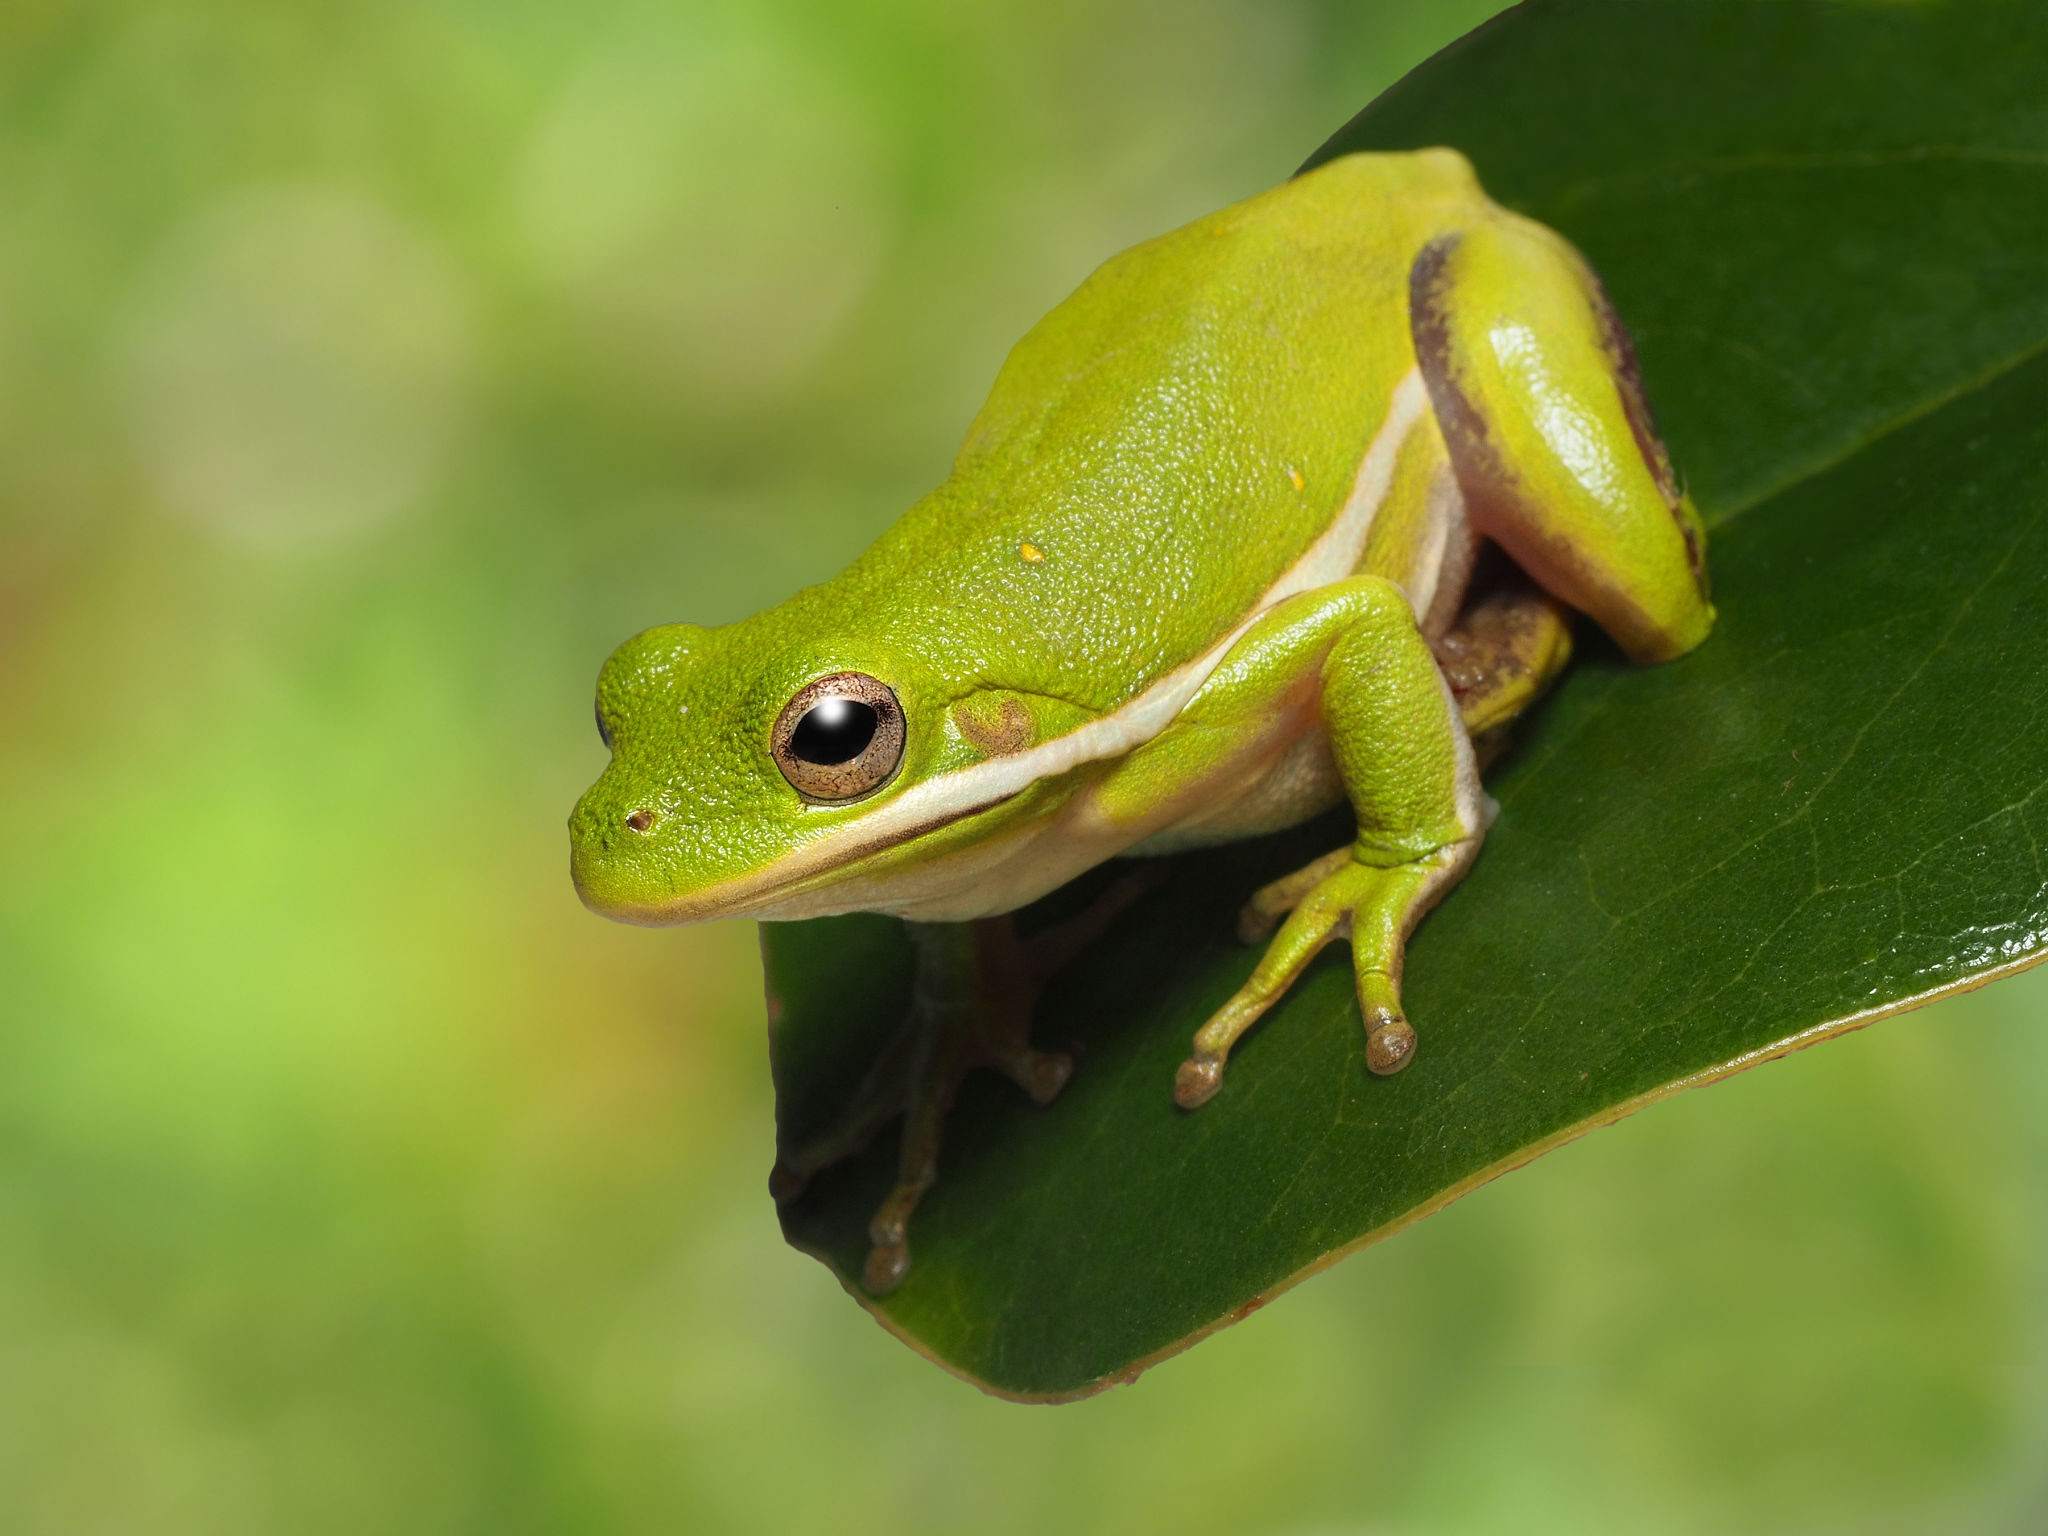
\includegraphics[width=0.4\textwidth, height=2in]{images/frog.png} 
  \end{center}
  \caption{Dimensions of each images in data ///// I couldn't find the full resolution image for the diagram so here's a frog}\label{fig:dimensions_of_each_image}
\end{figure*}

\hypertarget{initial-data-analysis}{%
\subsection{2.3 Initial Data Analysis}\label{initial-data-analysis}}

\begin{Shaded}
\begin{Highlighting}[]
\FunctionTok{library}\NormalTok{(dplyr)}
\FunctionTok{library}\NormalTok{(ggplot2)}
\FunctionTok{library}\NormalTok{(png)}

\DocumentationTok{\#\# change according to file path }
\NormalTok{folder\_path }\OtherTok{\textless{}{-}} \StringTok{"cell\_images"}
\NormalTok{clusters }\OtherTok{\textless{}{-}} \FunctionTok{paste0}\NormalTok{(}\StringTok{"cluster\_"}\NormalTok{, }\DecValTok{1}\SpecialCharTok{:}\DecValTok{28}\NormalTok{)}
\NormalTok{df }\OtherTok{\textless{}{-}} \FunctionTok{data.frame}\NormalTok{(}\AttributeTok{cluster =} \FunctionTok{character}\NormalTok{(),}
      \AttributeTok{num\_images =} \FunctionTok{integer}\NormalTok{(),}
      \AttributeTok{stringsAsFactors =} \ConstantTok{FALSE}\NormalTok{)}

\ControlFlowTok{for}\NormalTok{ (cluster }\ControlFlowTok{in}\NormalTok{ clusters) \{}
\NormalTok{  cluster\_path }\OtherTok{\textless{}{-}} \FunctionTok{file.path}\NormalTok{(folder\_path, cluster)}
\NormalTok{  num\_images }\OtherTok{\textless{}{-}} \FunctionTok{length}\NormalTok{(}\FunctionTok{list.files}\NormalTok{(cluster\_path,}
      \AttributeTok{pattern =} \StringTok{"\^{}cell\_.*}\SpecialCharTok{\textbackslash{}\textbackslash{}}\StringTok{.png$"}\NormalTok{))}
\NormalTok{  df }\OtherTok{\textless{}{-}}\NormalTok{ df }\SpecialCharTok{\%\textgreater{}\%} \FunctionTok{add\_row}\NormalTok{(}\AttributeTok{cluster =}\NormalTok{ cluster,}
      \AttributeTok{num\_images =}\NormalTok{ num\_images)\}}

\NormalTok{df }\OtherTok{\textless{}{-}}\NormalTok{ df }\SpecialCharTok{\%\textgreater{}\%} \FunctionTok{arrange}\NormalTok{(num\_images)}

\FunctionTok{ggplot}\NormalTok{(df, }\FunctionTok{aes}\NormalTok{(}\AttributeTok{x =} \FunctionTok{reorder}\NormalTok{(cluster, num\_images),}
      \AttributeTok{y =}\NormalTok{ num\_images)) }\SpecialCharTok{+}
  \FunctionTok{geom\_bar}\NormalTok{(}\AttributeTok{stat =} \StringTok{"identity"}\NormalTok{) }\SpecialCharTok{+}
  \FunctionTok{labs}\NormalTok{(}\AttributeTok{x =} \StringTok{"Cluster"}\NormalTok{, }\AttributeTok{y =} \StringTok{"Number of Images"}\NormalTok{) }\SpecialCharTok{+}
  \FunctionTok{theme}\NormalTok{(}\AttributeTok{axis.text.x =} \FunctionTok{element\_text}\NormalTok{(}\AttributeTok{angle =} \DecValTok{90}\NormalTok{,}
        \AttributeTok{vjust =} \FloatTok{0.5}\NormalTok{, }\AttributeTok{hjust=}\DecValTok{1}\NormalTok{)) }\SpecialCharTok{+}
  \FunctionTok{ggtitle}\NormalTok{(}\StringTok{"Number of Images in Each Cluster}
\StringTok{        (sorted by ascending order)"}\NormalTok{)}

\NormalTok{image\_data }\OtherTok{\textless{}{-}} \FunctionTok{data.frame}\NormalTok{(}\AttributeTok{Width =} \FunctionTok{numeric}\NormalTok{(),}
      \AttributeTok{Height =} \FunctionTok{numeric}\NormalTok{())}

\ControlFlowTok{for}\NormalTok{ (cluster\_num }\ControlFlowTok{in} \DecValTok{1}\SpecialCharTok{:}\DecValTok{28}\NormalTok{) \{}
\NormalTok{  cluster\_dir }\OtherTok{\textless{}{-}} \FunctionTok{paste0}\NormalTok{(}\StringTok{"cell\_images/cluster\_"}\NormalTok{,}
\NormalTok{        cluster\_num)}
  \ControlFlowTok{for}\NormalTok{ (file\_name }\ControlFlowTok{in} \FunctionTok{list.files}\NormalTok{(cluster\_dir,}
        \AttributeTok{pattern =} \StringTok{"\^{}cell\_}\SpecialCharTok{\textbackslash{}\textbackslash{}}\StringTok{d+}\SpecialCharTok{\textbackslash{}\textbackslash{}}\StringTok{.png$"}\NormalTok{,}
        \AttributeTok{full.names =} \ConstantTok{TRUE}\NormalTok{)) \{}
\NormalTok{    img }\OtherTok{\textless{}{-}} \FunctionTok{readPNG}\NormalTok{(file\_name)}
\NormalTok{    width }\OtherTok{\textless{}{-}} \FunctionTok{dim}\NormalTok{(img)[}\DecValTok{2}\NormalTok{]}
\NormalTok{    height }\OtherTok{\textless{}{-}} \FunctionTok{dim}\NormalTok{(img)[}\DecValTok{1}\NormalTok{]}
\NormalTok{    image\_data }\OtherTok{\textless{}{-}} \FunctionTok{rbind}\NormalTok{(image\_data,}
        \FunctionTok{data.frame}\NormalTok{(}\AttributeTok{Width =}\NormalTok{ width, }\AttributeTok{Height =}\NormalTok{ height))}
\NormalTok{  \}}
\NormalTok{\}}

\FunctionTok{ggplot}\NormalTok{(image\_data, }\FunctionTok{aes}\NormalTok{(}\AttributeTok{x =}\NormalTok{ Width, }\AttributeTok{y =}\NormalTok{ Height)) }\SpecialCharTok{+}
  \FunctionTok{geom\_point}\NormalTok{(}\AttributeTok{size =} \FloatTok{0.5}\NormalTok{) }\SpecialCharTok{+}
  \FunctionTok{xlab}\NormalTok{(}\StringTok{"Width"}\NormalTok{) }\SpecialCharTok{+}
  \FunctionTok{ylab}\NormalTok{(}\StringTok{"Height"}\NormalTok{) }\SpecialCharTok{+}
  \FunctionTok{ggtitle}\NormalTok{(}\StringTok{"Image Dimensions EDA"}\NormalTok{)}
\end{Highlighting}
\end{Shaded}

Figure \ref{fig:image_per_cluster} illustrates a notable trend in the
dataset, showing a gradual rise in the number of images as we move from
cluster 28 to cluster 1. Notably, the number of images in cluster 1 is
approximately ten times greater than that in cluster 28. This
observation highlights a substantial imbalance in the distribution of
clusters within the dataset, which should be taken into careful
consideration during the model training process. Figure
\ref{fig:dimensions_of_each_image} highlights varying dimensions of
images in the dataset, emphasising the need for proper resizing to
enable efficient feature extraction and representation.

\hypertarget{data-cleaning-and-preprocessing}{%
\subsection{2.4 Data cleaning and
preprocessing}\label{data-cleaning-and-preprocessing}}

In order to ensure standardised analysis, we first resize all images to
a resolution of 224 x 224 pixels. This step promotes compatibility with
pre-trained models and enhances computational efficiency during the
training process.

Additionally, we normalise each image by dividing the pixel values by
the 99th percentile to minimise any potential variations in pixel
intensity and ensure that the images have a standardised range of
values.

Furthermore, we apply masking techniques to generate clean images. By
removing pixels outside the cell boundaries, we isolate specific cells
of interest and reduce noise in the images. This masking process not
only improves the interpretability of the images but could also enhance
the accuracy of subsequent analysis and model training.

We save the raw and clean images separately with the same hierarchical
file structure. This approach maintains the integrity of the original
data while providing a cleaner version for further analysis. By
preserving this separation, we ensure that preprocessing steps do not
impact the original data and can be easily replicated and tracked.

\hypertarget{model-development}{%
\subsection{2.5 Model development}\label{model-development}}

\hypertarget{model-and-training-data-design}{%
\subsubsection{2.5.1 Model and training data
design}\label{model-and-training-data-design}}

We have chosen two neural architectures, Convolutional Neural Networks
(CNNs) and Transformers. CNNs are effective in capturing spatial
information and extracting hierarchical features from images, while
Transformers excel in modelling global context and dependencies within
images.

The raw and clean data are initially divided into train-validation and
test sets using an 80:20 split ratio and stratified sampling. However,
in this project, we specifically focus on exploring different sampling
methods to split train-validation data into 80:20, namely stratified and
independent sampling. The inclusion of stratified sampling in our
research is crucial to address significant data imbalances between
clusters and to examine the impact of a more balanced representation on
model performance.

We will develop a total of 8 models to investigate various combinations
of architectures, sampling methods, and types of data (raw and clean).
This comprehensive approach allows us to explore the effects of these
factors on the overall performance of the models.

\hypertarget{model-building-and-training}{%
\subsubsection{2.5.2 Model Building and
Training}\label{model-building-and-training}}

We employed pre-trained models (Resnet50V2 for CNN and Vision
Transformers for Transformers) to leverage existing knowledge, improve
efficiency and generalisation.

Resnet50V2, with its 50 layers and residual connections, enables
successful training of deep networks. In contrast, Vision Transformers
utilise transformers to capture global image relationships, facilitating
effective feature extraction and pattern recognition.

During training, we utilised a categorical cross-entropy loss function
to measure the discrepancy between predicted and actual class labels. We
trained the models for 30 epochs, which represents the number of
complete passes through the training dataset. Additionally, we selected
a batch size of 128, indicating the number of samples processed in each
iteration before updating the model's parameters. These choices aimed to
balance model convergence and computational time, optimising resource
usage while maintaining accurate gradient estimation and model
generalisation. We monitored the training process by analysing the
accuracy-epochs and loss-epochs plots to assess overfitting and
underfitting, an example of which can be found in Appendix A1 .

\emph{CNN} ResNet50V2 has 50 layers and includes convolutional blocks
with shortcut connections. These components allow the model to learn
intricate representations of input images by capturing important
features.

ResNet50V2 addresses the challenge of vanishing gradients in deep
networks by using residual blocks with skip connections. These
connections enable the model to effectively learn residual mappings,
capturing the differences between the input and desired output. This
design allows for successful training of deep models by improving
information flow.

For our image classification task, we customised ResNet50V2 by adjusting
its top layer and adding additional layers. The extracted features from
the convolutional blocks are processed through a global average pooling
layer to reduce their spatial dimensions. Dense layers with ReLU
activation, dropout regularisation, and a final dense layer with softmax
activation are applied. These layers generate classification
probabilities for the different image classes.

During classification, the network captures low-level features like
edges and textures in earlier layers, while deeper layers learn more
complex patterns and structures. The global average pooling layer
combines the features into a fixed-length representation, and subsequent
dense layers interpret this representation to produce class
probabilities using softmax activation. The predicted class label is
determined based on the highest probability.

\emph{Transformer} In vision transformers, 2D images are transformed
into sequences of patches, which are then processed by a transformer
architecture. This architecture utilises self-attention mechanisms to
capture relationships between patches, enabling the model to extract
meaningful representations from the image.

A key feature of vision transformers is the multi-head mechanism, which
allows the model to attend to multiple positions or patches
simultaneously. Each position has its own attention weights, which are
combined to capture a wide range of patterns and relationships within
the image. Feed-forward neural networks are also applied to each patch,
incorporating non-linear activations to capture complex relationships.

The transformer architecture consists of stacked transformer blocks,
connected through attention connections. This allows the model to
selectively focus on different parts of the input sequence during
generation.

Although primarily used for image classification, vision transformers
can generate probabilities for different image classes using a final
dense layer with softmax activation. These probabilities facilitate
classification based on the highest probability.

\hypertarget{model-optimisation}{%
\subsubsection{2.5.3 Model Optimisation}\label{model-optimisation}}

Each model was optimised until the validation accuracy surpassed the
threshold of 15\%, which is approximately 5 times the random guessing
probability of 1/28. The following optimization techniques were applied.

\hypertarget{evaluation}{%
\subsection{2.6 Evaluation}\label{evaluation}}

To evaluate the generalisation capabilities of our models, we used
unseen data to simulate real-world scenarios with new and unfamiliar
samples. This allowed us to assess the performance of our models in
accurately classifying unseen data and determining their ability to
generalise beyond the training set.

We selected accuracy as our primary quantitative evaluation metrics for
assessing model performance. We chose these metrics due to their
simplicity and ease of interpretation. To compare the performance of
different models, we utilised side-by-side bar plots to visualise the
accuracy values.

As our second evaluation metric, we employed the confusion matrix, which
offers valuable insights into the classification performance of our
models. This matrix allows us to analyse the accuracy of each cluster,
identify misclassifications across different clusters, and assess any
imbalances or biases present in the classification results.

We employed innovative evaluation strategies such as Gradient-weighted
Class Activation Mapping (Grad-CAM) for CNN and Spatially Adaptive
Activation Value(SAAV) for Transformers to enhance interpretability.
These techniques allowed us to visualise where the models focused their
attention in the images. By validating the activations, we assessed if
the models correctly identified relevant patterns. Deviations from
expected patterns indicated potential areas for improvement, such as
further training or data collection efforts to enhance pattern
understanding (Team, n.d.).

We also evaluate on models storage requirements to optimise resource
allocation and minimise the storage resources needed for deploying and
running the models, thus enhancing cost-effectiveness.

During the model selection process, we initially prioritised accuracy
and the confusion matrix as performance metrics. Additionally, we
utilised Grad-CAM and SAAV techniques to assess the interpretability of
the models. If a model demonstrated higher interpretability by correctly
focusing on the relevant regions of the input data, it was considered a
potential candidate, even if its accuracy was slightly lower compared to
other models. Furthermore, in cases where there was a significant
difference in storage requirements between two architectures, we
favoured the architecture with smaller storage needs.

This approach allowed us to choose a final model that struck a balance
between satisfactory accuracy, interpretability, and cost-effectiveness.
These factors were deemed important for our stakeholders and contributed
to the overall success of our methodology.

\hypertarget{results}{%
\section{3. Results}\label{results}}

\hypertarget{performance-metrics}{%
\subsection{3.1 Performance metrics}\label{performance-metrics}}

\begin{Shaded}
\begin{Highlighting}[]
\FunctionTok{library}\NormalTok{(ggplot2)}

\NormalTok{dir }\OtherTok{\textless{}{-}} \StringTok{"Biotechnology/Model\_result/"}

\NormalTok{outputs }\OtherTok{\textless{}{-}} \FunctionTok{list}\NormalTok{(}
  \StringTok{"output\_clean\_independent\_cnn.csv"}\NormalTok{,}
  \StringTok{"output\_raw\_independent\_cnn.csv"}\NormalTok{,}
  \StringTok{"output\_clean\_stratified\_cnn.csv"}\NormalTok{,}
  \StringTok{"output\_raw\_stratified\_cnn.csv"}\NormalTok{,}
  \StringTok{"output\_clean\_independent\_transformers.csv"}\NormalTok{,}
  \StringTok{"output\_raw\_independent\_transformers.csv"}\NormalTok{,}
  \StringTok{"output\_clean\_stratified\_transformers.csv"}\NormalTok{,}
  \StringTok{"output\_raw\_stratified\_transformers.csv"}
\NormalTok{)}

\NormalTok{read\_csv }\OtherTok{\textless{}{-}} \ControlFlowTok{function}\NormalTok{(f) \{ }
  \FunctionTok{read.csv}\NormalTok{(}\FunctionTok{paste0}\NormalTok{(dir, f))}
\NormalTok{\}}

\NormalTok{output }\OtherTok{\textless{}{-}} \FunctionTok{lapply}\NormalTok{(outputs, read\_csv)}

\NormalTok{accu }\OtherTok{\textless{}{-}} \ControlFlowTok{function}\NormalTok{(o) \{ }\FunctionTok{unique}\NormalTok{(o}\SpecialCharTok{$}\NormalTok{Test.Accuracy) \}}

\NormalTok{accuracy }\OtherTok{\textless{}{-}} \FunctionTok{lapply}\NormalTok{(output, accu)}

\NormalTok{Test }\OtherTok{\textless{}{-}} \FunctionTok{data.frame}\NormalTok{(}
  \AttributeTok{Model =} \FunctionTok{factor}\NormalTok{(}\FunctionTok{c}\NormalTok{(}
    \StringTok{"Independent/Clean"}\NormalTok{, }\StringTok{"Independent/Raw"}\NormalTok{,}
    \StringTok{"Stratified/Clean"}\NormalTok{, }\StringTok{"Stratified/Raw"}\NormalTok{,}
    \StringTok{"Independent/Clean"}\NormalTok{, }\StringTok{"Independent/Raw"}\NormalTok{,}
    \StringTok{"Stratified/Clean"}\NormalTok{, }\StringTok{"Stratified/Raw"}
\NormalTok{  )),}
  \AttributeTok{Architecture =} \FunctionTok{factor}\NormalTok{(}\FunctionTok{c}\NormalTok{(}
    \StringTok{"CNN"}\NormalTok{, }\StringTok{"CNN"}\NormalTok{, }\StringTok{"CNN"}\NormalTok{, }\StringTok{"CNN"}\NormalTok{,}
    \StringTok{"Tranformers"}\NormalTok{, }\StringTok{"Tranformers"}\NormalTok{,}
    \StringTok{"Tranformers"}\NormalTok{, }\StringTok{"Tranformers"}
\NormalTok{  )),}
  \AttributeTok{Accuracy =} \FunctionTok{unlist}\NormalTok{(accuracy)}
\NormalTok{)}

\NormalTok{p1 }\OtherTok{\textless{}{-}} \FunctionTok{ggplot}\NormalTok{(}\AttributeTok{data =}\NormalTok{ Test) }\SpecialCharTok{+}
  \FunctionTok{geom\_bar}\NormalTok{(}
    \FunctionTok{aes}\NormalTok{(}\AttributeTok{x =}\NormalTok{ Model, }\AttributeTok{y =}\NormalTok{ Accuracy,}
        \AttributeTok{fill =}\NormalTok{ Architecture),}
    \AttributeTok{stat =} \StringTok{"identity"}\NormalTok{, }\AttributeTok{position =} \StringTok{"dodge"}
\NormalTok{  ) }\SpecialCharTok{+}
  \FunctionTok{labs}\NormalTok{(}
    \AttributeTok{title =} \StringTok{"Test Accuracy by Model"}\NormalTok{,}
    \AttributeTok{x =} \StringTok{"Training Data"}\NormalTok{,}
    \AttributeTok{y =} \StringTok{"Accuracy"}
\NormalTok{  ) }\SpecialCharTok{+}
  \FunctionTok{theme}\NormalTok{(}\AttributeTok{axis.text.x =}
          \FunctionTok{element\_text}\NormalTok{(}\AttributeTok{angle =} \DecValTok{45}\NormalTok{, }\AttributeTok{hjust =} \DecValTok{1}\NormalTok{)) }\SpecialCharTok{+} 
  \FunctionTok{scale\_fill\_brewer}\NormalTok{(}\AttributeTok{palette =} \StringTok{"Set3"}\NormalTok{)}

\FunctionTok{suppressMessages}\NormalTok{(}\FunctionTok{ggsave}\NormalTok{(}\StringTok{"accuracies.pdf"}\NormalTok{, p1))}
\end{Highlighting}
\end{Shaded}

\begin{figure*}
  \begin{center}
    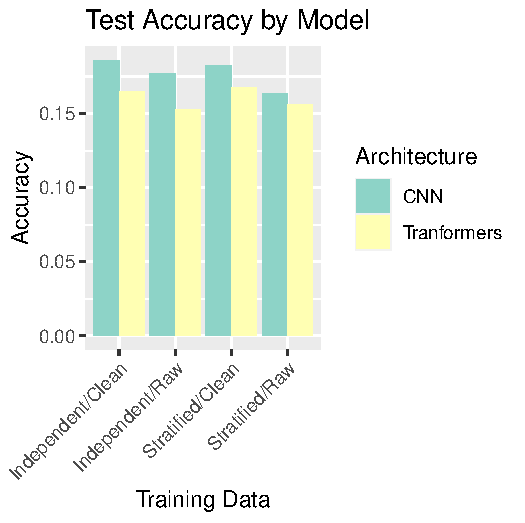
\includegraphics[width=4in, height=4in]{accuracies.pdf} 
  \end{center}
  \caption{Wide ggplot2 figure}\label{fig}
\end{figure*}

\begin{table}[h]
\begin{tabular}{l|l|l|l}
Architecture & Sampling Method & Data Types & Accuracy (\%) \\ \hline
Transformers & Stratified      & Clean      & 16.78         \\ \cline{3-4} 
             &                 & Raw        & 15.25         \\ \cline{2-4} 
             & Independent     & Clean      & 16.49         \\ \cline{3-4} 
             &                 & Raw        & 15.64         \\ \hline
CNN          & Stratified      & Clean      & 18.22         \\ \cline{3-4} 
             &                 & Raw        & 16.32         \\ \cline{2-4} 
             & Independent     & Clean      & 18.61         \\ \cline{3-4}
             &                 & Raw        & 17.69        
\end{tabular}
\caption{\label{tab:acc_table} Accuracy comparisons between models}
\end{table}

This \emph{pinp is not PNAS} template started when the introduction to
\href{http://dirk.eddelbuettel.com/code/rcpp.html}{Rcpp} by
\cite{PeerJ:Rcpp} was converted into this updated
\href{https://eddelbuettel.github.io/pinp/Rcpp-introduction.pdf}{Rcpp
Introduction} vignette. It is based on the
\href{https://github.com/rstudio/rticles/tree/master/inst/rmarkdown/templates/pnas_article}{pnas\_article}
template of the wonderful
\href{https://cran.r-project.org/package=rticles}{rticles} package by
\cite{CRAN:rticles}. The conversion from markdown to latex is
facilitated by
\href{https://cran.r-project.org/package=rmarkdown}{rmarkdown}
\citep{CRAN:rmarkdown} and
\href{https://cran.r-project.org/package=knitr}{knitr}
\citep{CRAN:knitr}. The underlying LaTeX macros are from
\href{http://www.pnas.org/site/authors/latex.xhtml}{pnas.org}.

The remainder of the document carries over from the corresponding
\href{https://github.com/rstudio/rticles/tree/master/inst/rmarkdown/templates/pnas_article}{pnas\_article}
template document. but has been edited and updated to our use case. A
few specific tips follow. In general, for fine-tuning some knowledge of
LaTeX is helpful.

\hypertarget{author-affiliations}{%
\subsection{Author Affiliations}\label{author-affiliations}}

Per common academic best practice, you can include your department,
institution, and complete address, with the ZIP/postal code, for each
author. Use lower case letters to match authors with institutions, as
shown in the example. Authors with an ORCID ID may supply this
information at submission.

\hypertarget{document-options}{%
\subsection{Document Options}\label{document-options}}

We support several options via the YAML header

\begin{itemize}
\tightlist
\item
  Setting a DOI or URL footer, for example for the CRAN package URL,
  which is placed in the bottom-left footer of the title page and even
  pages;
\item
  Setting a footer label, for example \emph{YourPackage Vignette}
  stating your package, which is placed in the bottom-right footer on
  odd pages;
\item
  Setting a free-form author field used on the inside footer;
\item
  Optional \emph{Draft} watermark to be added to each page;
\item
  Line of custom text in subtitle (\texttt{date\_subtitle}) suitable to
  give publication info of the draft, e.g.~journal name in a post-print;
\item
  Document date that appears in the footer can be specified manually
  using \texttt{document\_date}.
\end{itemize}

\hypertarget{references}{%
\subsection{References}\label{references}}

Here we differ from PNAS and suggest natbib. References will appear in
author-year form. Use \texttt{\textbackslash{}citet\{\}},
\texttt{\textbackslash{}citep\{\}}, etc as usual.

We default to the \texttt{jss.bst} style. To switch to a different
bibliography style, please use \texttt{biblio-style:\ style} in the YAML
header.

\hypertarget{inline-r-code}{%
\subsection{Inline R Code}\label{inline-r-code}}

The PNAS sample included a fixed PNG image here, but this document
prefers to show the results and embedding of \emph{R} code.

\begin{Shaded}
\begin{Highlighting}[]
\FunctionTok{library}\NormalTok{(ggplot2)}
\FunctionTok{ggplot}\NormalTok{(mtcars, }\FunctionTok{aes}\NormalTok{(wt, mpg)) }\SpecialCharTok{+}
    \FunctionTok{geom\_point}\NormalTok{(}\AttributeTok{size=}\DecValTok{3}\NormalTok{, }\FunctionTok{aes}\NormalTok{(}\AttributeTok{colour=}\FunctionTok{factor}\NormalTok{(cyl))) }\SpecialCharTok{+}
    \FunctionTok{theme}\NormalTok{(}\AttributeTok{legend.position=}\StringTok{"none"}\NormalTok{)}
\end{Highlighting}
\end{Shaded}

\begin{figure}

{\centering 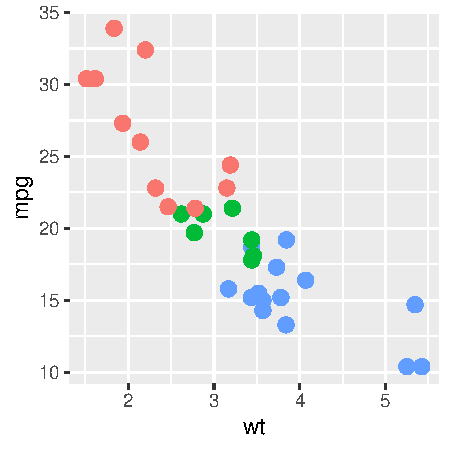
\includegraphics{DATA3888_Final_report_files/figure-latex/figex-1} 

}

\caption{Narrow ggplot2 figure}\label{fig:figex}
\end{figure}

Here we use a standard knitr bloc with explicit options for

\begin{itemize}
\tightlist
\item
  figure width and height (\texttt{fig.width}, \texttt{fig.height}),
  both set to three inches;
\item
  whether the code is shown (\texttt{echo=TRUE}); and
\item
  the caption (\texttt{fig.cap}) as shown above.
\end{itemize}

\hypertarget{single-column-equations}{%
\subsection{Single column equations}\label{single-column-equations}}

Authors may use 1- or 2-column equations in their article, according to
their preference.

To allow an equation to span both columns, options are to use the
\texttt{\textbackslash{}begin\{figure*\}...\textbackslash{}end\{figure*\}}
environment mentioned above for figures. The
\texttt{\textbackslash{}begin\{widetext\}...\textbackslash{}end\{widetext\}}
environment as shown in equation \ref{eqn:example} below is deprecated,
but \LaTeX commands \texttt{\textbackslash{}onecolumn} and
\texttt{\textbackslash{}twocolumn} work fine.

Please note that this option may run into problems with floats and
footnotes, as mentioned in the \href{http://texdoc.net/pkg/cuted}{cuted
package documentation}. In the case of problems with footnotes, it may
be possible to correct the situation using commands
\texttt{\textbackslash{}footnotemark} and
\texttt{\textbackslash{}footnotetext}.

\begin{equation}
  \begin{aligned}
(x+y)^3&=(x+y)(x+y)^2\\
       &=(x+y)(x^2+2xy+y^2) \\
       &=x^3+3x^2y+3xy^3+x^3. 
       \label{eqn:example} 
  \end{aligned}
\end{equation}

\hypertarget{appendix}{%
\section{Appendix}\label{appendix}}

\begin{Shaded}
\begin{Highlighting}[]
\NormalTok{history }\OtherTok{\textless{}{-}} \FunctionTok{read.csv}\NormalTok{(}
  \StringTok{"Biotechnology/History/c\_i\_cnn.csv"}
\NormalTok{)}

\FunctionTok{library}\NormalTok{(ggplot2)}

\NormalTok{custom\_colors }\OtherTok{\textless{}{-}} \FunctionTok{c}\NormalTok{(}\StringTok{"blue"}\NormalTok{, }
                   \StringTok{"red"}\NormalTok{)}
\NormalTok{custom\_labels }\OtherTok{\textless{}{-}} \FunctionTok{c}\NormalTok{(}\StringTok{"Train"}\NormalTok{, }
                   \StringTok{"Validation"}\NormalTok{)}

\FunctionTok{ggplot}\NormalTok{(}\AttributeTok{data =}\NormalTok{ history) }\SpecialCharTok{+}
  \FunctionTok{geom\_line}\NormalTok{(}\FunctionTok{aes}\NormalTok{(}\AttributeTok{x =}\NormalTok{ epoch, }
                \AttributeTok{y =}\NormalTok{ train\_accuracy, }
                \AttributeTok{color =} \StringTok{"Train"}\NormalTok{)) }\SpecialCharTok{+}
  \FunctionTok{geom\_line}\NormalTok{(}\FunctionTok{aes}\NormalTok{(}\AttributeTok{x =}\NormalTok{ epoch, }
                \AttributeTok{y =}\NormalTok{ validation\_accuracy, }
                \AttributeTok{color =} \StringTok{"Validation"}\NormalTok{)) }\SpecialCharTok{+}
  \FunctionTok{scale\_color\_manual}\NormalTok{(}\AttributeTok{values =}\NormalTok{ custom\_colors, }
                     \AttributeTok{labels =}\NormalTok{ custom\_labels) }\SpecialCharTok{+}
  \FunctionTok{labs}\NormalTok{(}\AttributeTok{x =} \StringTok{"Epoch"}\NormalTok{, }
       \AttributeTok{y =} \StringTok{"Accuracy"}\NormalTok{,}
       \AttributeTok{colour =} \StringTok{""}\NormalTok{) }\SpecialCharTok{+}
  \FunctionTok{theme\_bw}\NormalTok{()}
\end{Highlighting}
\end{Shaded}

\begin{figure}

{\centering 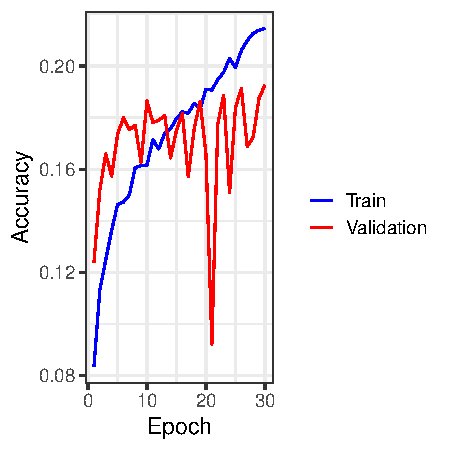
\includegraphics{DATA3888_Final_report_files/figure-latex/cnn_independent_graph_acc-1} 

}

\caption{Model accuracy for CNN Independent/clean}\label{fig:cnn_independent_graph_acc}
\end{figure}

\begin{Shaded}
\begin{Highlighting}[]
\FunctionTok{ggplot}\NormalTok{(}\AttributeTok{data =}\NormalTok{ history) }\SpecialCharTok{+}
  \FunctionTok{geom\_line}\NormalTok{(}\FunctionTok{aes}\NormalTok{(}\AttributeTok{x =}\NormalTok{ epoch, }
                \AttributeTok{y =}\NormalTok{ loss, }
                \AttributeTok{color =} \StringTok{"Train"}\NormalTok{)) }\SpecialCharTok{+}
  \FunctionTok{geom\_line}\NormalTok{(}\FunctionTok{aes}\NormalTok{(}\AttributeTok{x =}\NormalTok{ epoch, }
                \AttributeTok{y =}\NormalTok{ validation\_loss, }
                \AttributeTok{color =} \StringTok{"Validation"}\NormalTok{)) }\SpecialCharTok{+}
  \FunctionTok{scale\_color\_manual}\NormalTok{(}\AttributeTok{values =}\NormalTok{ custom\_colors, }
                     \AttributeTok{labels =}\NormalTok{ custom\_labels) }\SpecialCharTok{+}
  \FunctionTok{labs}\NormalTok{(}\AttributeTok{x =} \StringTok{"Epoch"}\NormalTok{, }
       \AttributeTok{y =} \StringTok{"Loss"}\NormalTok{, }
       \AttributeTok{title =} \StringTok{"Model Loss"}\NormalTok{, }
       \AttributeTok{colour =} \StringTok{""}\NormalTok{) }\SpecialCharTok{+}
  \FunctionTok{theme\_bw}\NormalTok{()}
\end{Highlighting}
\end{Shaded}

\begin{figure}

{\centering 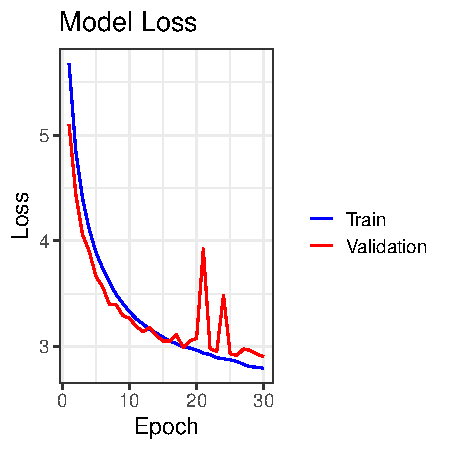
\includegraphics{DATA3888_Final_report_files/figure-latex/cnn_independent_graph_loss-1} 

}

\caption{Model loss for CNN Independent/clean}\label{fig:cnn_independent_graph_loss}
\end{figure}

\begin{figure}
\begin{center}
  \centering
  \begin{minipage}[b]{0.8\textwidth}
    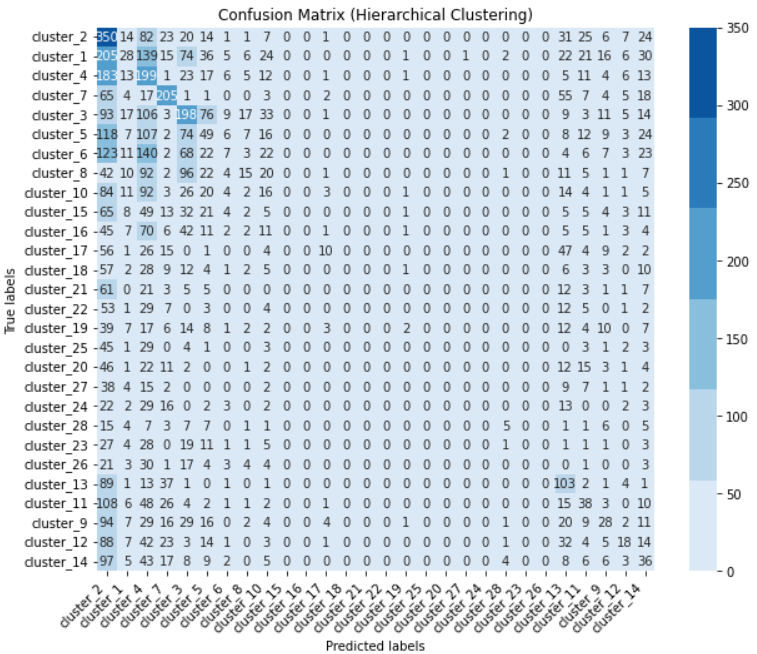
\includegraphics[width=\textwidth]{images/Confusion_Matrix/Cmax_CNN_Stratified_Clean.png}
    \caption{Flower one.}
  \end{minipage}
  \hfill
  \begin{minipage}[b]{0.8\textwidth}
    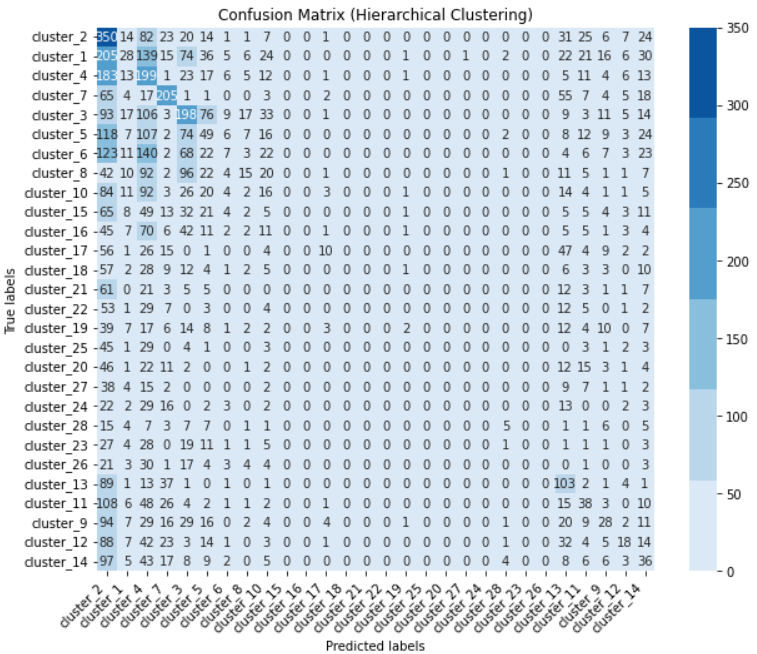
\includegraphics[width=\textwidth]{images/Confusion_Matrix/Cmax_CNN_Stratified_Clean.png}
    \caption{Flower two.}
  \end{minipage}
  
\end{center}
\end{figure}

%\showmatmethods
\showacknow


\bibliography{pinp}
\bibliographystyle{jss}



\end{document}
